\documentclass{article}
\usepackage[utf8]{inputenc}
\usepackage{graphicx}
\graphicspath{ {images/} }
\usepackage{enumitem}

%----------------------------------------------------------------------------------------
%	TITLE PAGE
%----------------------------------------------------------------------------------------

\newcommand*{\titleGP}{\begingroup
\centering 
\vspace*{\baselineskip}

\rule{\textwidth}{1.6pt}\vspace*{-\baselineskip}\vspace*{2pt}
\rule{\textwidth}{0.4pt}\\[\baselineskip]

{\LARGE CGIS Map Production\\ [0.3\baselineskip] Architectural Design} \\ [0.2\baselineskip]
\rule{\textwidth}{0.4pt}\vspace*{-\baselineskip}\vspace{3.2pt}
\rule{\textwidth}{1.6pt}\\[\baselineskip] %

% \scshape %
% A concise specification on the functional requirements  \\
% and use cases of CGIS \\[\baselineskip]

% \vspace*{2\baselineskip}

Compiled By \\[\baselineskip]
{\Large Siyabonga Magubane - u15289347 \\ Bernard van Tonder -  u15008992 \\ Boikanyo Modiko - u15227678 \\ Cian Steenkamp - u15095682 \\ Robert Trankle - u15092454\par} 

\vfill

{\scshape 2017} \\[0.3\baselineskip]
{\large \#include}\par

\endgroup}

\begin{document}
	\begin{center}
		\includegraphics[width=\textwidth]{front-page}
	\end{center}
\titleGP
\tableofcontents
\listoffigures
\newpage
\section{Introduction}
{This chapter of the document is used to identify the Purpose of the document, as well as all references used.}
	\subsection{Purpose}
    {The main purpose of this document is to identify eah sub-system of the CGIS Map production system. It will address the architectural design of each subsystem, by using design patterns and models to conceptualize and visualize the system.
    \\\\
    The choice of technologies, will also be provided.}
   
 \section{Module Design}
 	\subsection{Access Module}
       \begin{figure}[h!]
        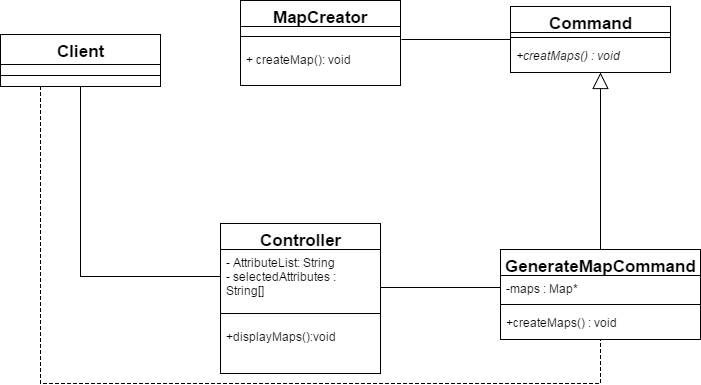
\includegraphics[width=\textwidth]{AccessCD}
            \caption{Access subsystem Class Diagram}
        \end{figure}
        
The above diagram represents the class diagram of the Access subsystem. This subsystem is used to facilitate the communication between the other subsystems on the server side, and the user on the client side.\\\\
        The design pattern used was the Command pattern. It was chosen because it allows for the encapsulation of a request as an object. Thereby allowing the system parameterize clients with different requests, which would be the different attributes chosen.
        \\\\
        The Controller class is used to communicate directly with the client, and display the maps once they have been generated.
        \\\\
        The MapCreator class is linked to the generate Maps subsystem, and is part of that system. It is the link between the two subsystems, and is summarized just to show the relation.
        \\\\
        The GenerateMapCommand is the concrete class of the Command class(which is a virtual class). It contains an array of Maps which will be generated and the function call to create the Maps.
        \\\\
     
     
       \begin{figure}[h!]
        \includegraphics[width=\textwidth]{access_sequence_diagram}
            \caption{Access subsystem Sequence Diagram}
        \end{figure}
        
The figure above depicts the sequence diagram for the access subsystem. The sequence diagram illustrates the sequence of interaction amongst objects (or classes). The Controller class/object will call displayMaps() which will invoke the generateMapCommand object which in turn calls the createMaps() function which represents the factory method used to generate/prepare the thematic maps. The generated map(s) will then be returned.          
 \\\\
     \newpage
     \begin{figure}[h!]
       \includegraphics[width=\textwidth] {access_activity_diagram2}
       \caption{Access subsystem Activity Diagram}
       \end{figure}
       \newpage
The activity diagram above models the flow control from one activity to another. The activity diagram models the activity flow of the system. If the user is an administrator then he/she will need to login in order to be able to update the database (CRUD). Any user (administrator or normal user) can then select the attributes to be used to generate the thematic maps. Once the user selected the attributes he/she can click the "Display Maps" button to generate the 3 thematic maps.  
\\\\      
		\begin{figure}[h!]
       \includegraphics[width=\textwidth] {map_display_and_scaling_use_case}
       \caption{Access subsystem Use Case Diagram}
       \end{figure}
       \newpage
       \subsection{Database Manager Module}
      
        \begin{figure}[h!]
        \includegraphics[width=\textwidth]{DBManage_class_diagram}
        	\caption{Database Manager subsystem Class Diagram}
            \end{figure}
     
The above diagram represents the class diagram of the database Module subsystem. This subsystem is used to facilitate communication between the other database module and the other subsystems.
 \\\\
The design pattern used in this module is the state design pattern. The Database Manager class is the State class, Enquire is the context class and the add, delete and update are the ConcreteState classes. Enquire sends a request to the data base manager and the data base manager updates the dataset. 
\\\\
\newpage
	\begin{figure}[h!]
    \includegraphics[width=\textwidth]{DBManager_Sequence_Diagram}
    \caption{Database Manager subsystem Sequence Diagram}
    \end{figure}
   
  The figure above depicts the sequence diagram for the Database Manager subsystem. The sequence diagram illustrates the sequence of interaction amongst classes.
  
    \begin{figure}[h!]
     \centering  \includegraphics[width=\textwidth, height=7cm, keepaspectratio]{DBM_ActivityDiagram}
     \caption{Database Manager subsystem Activity Diagram}
    \end{figure}
    The behavior of the Database Manager depends on its state. The state is set, and the relevant action is executed.
    \begin{figure}[h!]
     \centering  \includegraphics[width=\textwidth, height=7cm, keepaspectratio]{DBM_UCD}
     \caption{Database Manager subsystem Use Case Diagram}
    \end{figure}
    
\pagebreak     
       \subsection{Map design Module}
        \begin{figure}[h!]
        \includegraphics[width=\textwidth]{map_design_class_diagram}
        	\caption{Map design Class Diagram}
            \end{figure}
            
The above diagram represents the class diagram of the map design subsystem. This subsystem is used generate the thematic maps.
\\\\
The design patterns used were the Factory Method, Builder pattern, and the Strategy pattern.
\\\\
The Factory method defines an interface for creating maps.
\\\\
The Builder pattern allows multiple classes to help in the creation of mapBuilder objects. The strategy allows the definition of a family of classificationMethod algorithms, encapsulates each one, and makes them interchangeable. 
\\\\
The Strategy pattern allows the standidisationMethod to vary independently from the clients that use it.
\\\\            
            
         \begin{figure}[h!]
        \includegraphics[width=\textwidth]{map_design_sequence_diagram}
        	\caption{Map design Sequence Diagram}
            \end{figure}
The figure above depicts the sequence diagram for the map design module. The sequence diagram illustrates the sequence of interaction amongst objects (or classes).
                       \newpage
            \begin{figure}[h!]
	\centering
	\includegraphics[width=.5\textwidth]{flow_diagram}
	\caption{Map design Activity Diagram}
\end{figure}

The figure above depicts the activity diagram for the map design module. The user has an option to link their own database to the system or use the data which has already been provided.
\\\\
After specifying the data that will be used, the user can then select which attributes they would like their maps to contain. Based on the attributes selected, the system will generate three different thematic maps for the user to view.
\\\\
The user can then save the specific maps by downloading them in a format of their choice.
\\\\
This process can repeated for as many times the user deems necessary.
              
 \newpage   
            \begin{figure}[h!]
	\centering
	\includegraphics[width=.9\textwidth]{gen_maps2}
	\caption{Map design Use Case}
\end{figure}
            
  \newpage          
    \section{System Assessment}
    	\subsection{Deployment Diagram}
        
        \begin{figure}[h!]
        \includegraphics[width=\textwidth]{CGIS-Deployment}
            \caption{CGIS Deployment Diagram}
        \end{figure}
        
        \subsection{Technologies Used}
        {The technologies used will include a range of languages and Open Source Software.\\\\
        The following key technologies have been identified, in which the team deems applicable to the purpose of the system :
        \begin{itemize}
        \item OpenLayers : Is an open source JavaScript library for displaying geospatial data in web browsers.
        \item GeoServer :  Is an open source server for sharing geospatial data. Designed for interoperability, it publishes data from any major spatial data source using open standards.
        \item Eclipse Jetty : is a Java HTTP (Web) server and Java Servlet container.
        \item PostGIS : It will be used to manage and edit the Geospatial data which the admin will be able to manage, through the Database Management subsystem.
        \item HTML/CSS/Bootstrap : All of the following languages pertain to the creation of the front end of the system. It will be used to create the user interface, where users will be able to interact with the system.
        \item jQuery : jQuery is a fast, small, and feature-rich JavaScript library. It makes things like HTML document traversal and manipulation, event handling, animation, and Ajax much simpler with an easy-to-use API that works across a multitude of browsers.
        
        \end{itemize}}

\newpage
\section{References}
{Source Making. 2017. Design Patterns. [ONLINE] Available at: https://www.sourcemaking.com/. [Accessed 19 June 2017].}
         
\end{document}
